\documentclass[a4paper,12pt]{article}
\usepackage{graphicx}
\usepackage{hyperref}
\usepackage[margin=1in]{geometry}

\title{Quasi-Experiments sLab}
\author{}
\date{}

\begin{document}

\maketitle

\vspace{-4em}

\begin{enumerate}\itemsep0.5em

\section*{Instrumental Variables}

\item Load the \texttt{Smoking.dta} data (from Blackboard). This is a very small dataset containing information about cigarette consumption, prices, and taxes for 48 U.S. states.

\item Start by summarizing the variables using tables or graphs.

\item Create logged transformations of some key variables:\\
\texttt{gen logpacks = log(packs)\\
gen logrprice = log(rprice)\\
gen logincome = log(income)}

You should use the logged forms of these variables in the following analyses.

\item Our goal is to estimate the effect of logged cigarette prices (\textbf{logrprice}) on smoking rates (\textbf{logpacks}). Construct an OLS estimate of this effect.

\subsection*{Finding instruments}

\item State-level cigarette prices and smoking rates may be influenced by many things. Draw a causal graph of this causal relationship along with any confounding variables. Where would you put an instrumental variable to help identify an effect?

\item Some authors have suggested state-level cigarette tax rates (\textbf{tax}) could be a valid instrument. Does this seem like a {\em credibly exogenous} instrument for this problem?

\item Others have suggested that a better instrument is the amount of VAT (general sales tax on all purchased goods; \textbf{tdiff}) is a better instrument. Does this seem like a {\em credibly exogenous} instrument? Is it more or less so than cigarette-specific taxes?

\item Test whether cigarette-specific and general tax rates are {\em relevant} instruments. Are they strong or weak instruments?

\subsection*{Two-stage least squares estimation}

\item Let's assume that \textbf{tdiff} is a credible instrument. Manually generate a two-stage least squares estimate by regressing (using \texttt{reg}) logged cigarette prices on \textbf{tdiff}. Based on this first stage equation, do general sales taxes seem to be a strong instrument?

\item Save the fitted values from this regression as a new variable \textbf{pricefit}.

\item Manually estimate the second stage equation using \textbf{pricefit} to predict \textbf{logpacks}. How does the estimate compare to your OLS estimate from above?

\item Remember that the SEs calculated in this method are incorrect. To obtain correct SEs, we need to use the \texttt{ivregress} command. It has the following syntax:\\
\texttt{ivregress 2sls outcome [exogenousvarlist] (endogenousvarlist = ivlist)}

How do coefficient estimates and SEs from \texttt{ivregress} compare to the estimates from manually performing two-stage least squares?

\subsection*{First-stage diagnostics}

\item To include additional details in the output, we can specify some options when we call \texttt{ivregress}. Add the \texttt{, first} option and compare the output to the output from your manual estimation of the first stage.

\item You can also use \texttt{estat firststage} to instead just report summary statistics for the first stage without the coefficient estimates. Note how much of the output from \texttt{estat firststage} is the same as the summary statistics we obtain from any regression. The key statistic here is the F-statistic. Recall that in a regression with one regressor, the F-statistic is simply the square of the t-statistic for the coefficient. A rule-of-thumb is that an F-statistic greater than 10 is required for the instrument to be considered strong.

\item The bottom half of the \texttt{estat firststage} output is something new. It lists critical values (in F-statistic terms) above which we can reject a null hypothesis of having a weak instrument(s). Does the F-statistic exceed these critical values?

\subsection*{Tests of endogeneity}

\item While we cannot test the exclusion restriction (that the instrument has no direct effect on the outcome), we can test whether the seemingly endogenous regressor is in fact endogenous. We do this by comparing the OLS estimates of the regressor's effects to those estimated by 2SLS. Or, to put it another way, we see whether the portion of $X$ not explained by the instrument has any independent effect on $Y$. Stata provides this test --- called the Durbin-Wu-Hausman Test --- using \texttt{estat endogenous}. We are interested in the last line of output, which provides an F-statistic and associated p-value for a test of the null hypothesis that the included covariates in the second stage are exogenous. Rejecting the null would indicate that the include variable(s) are endogenous and should be instrument. We have one included variable (\texttt{logrprice}). Does it seem to be exogenous?

\item To get a feel for what's happening in the DWH test, let's calculate it manually. First, rerun the first-stage regression. Then save the residuals from the firststage as a new variable \textbf{resid}. Now regress \textbf{logpacks} on \textbf{logrprice} and \textbf{resid}. If you run \texttt{test resid}, the F-statistic and p-value should match those of from the output of \texttt{estat endogenous}.


\subsection*{Covariates in IV estimation}

\item We don't simply need to estimate a model with one endogenous regressor and one instrument. We can also include additional covariates in our model. Perhaps there were other variables that we think confound the relationship between \textbf{logrprice} and \textbf{logpacks} and that we were able to observe directly. We can include these in our model. For example, maybe we think that state income \textbf{logincome} has an effect on smoking. Estimate a two-stage least squares model that includes this as an additional covariate. Does it seem to be influential?

\item To get a handle on what happens when we include additional covariates in our model, run the following:\\
\texttt{quietly reg logrprice tdiff logincome\\
predict pricefit2\\
reg logpacks pricefit2 logincome}

Here we manually calculate the two-stage least squares estimates, as we did above. Note how we include \textbf{logincome} in both the first- and second-equations. The reason for this that we when we regress $X$ on the instrument and all of the other covariates, the residuals from that first-stage model are --- by definition --- independent of the instrument and the covariates. Thus when we estimate the second-stage equation using the instrument $\hat{X}$, we leave some of the original variation from $X$ in the second-stage error term, but that variation is independent of $\hat{X}$ and the other covariates.

\subsection*{Multiple instruments}

\item What if we happen to be in the rare situation where we have multiple instruments? Well, they allow us to additional conduct tests of ``overidentifying restrictions.'' This is a test of the null hypothesis that all instruments are valid. Rejecting it suggests that at least one of the instruments is invalid. Try running a 2SLS estimation using \texttt{population} as an additional instrument. Then use the \texttt{estat overid} to test the validity of the combined instruments. 

\item In practice, we will rarely have one instrument let alone two or more. As such, we are restricted to a world where there is only one included variable that is affected by unobserved confounding. Having two instruments would mean we could estimate a model with two endogenous regressors if both instruments are credibly exogenous for both of these variables. Feel free to estimate such a model.

\subsection*{Model fit and specification}

\item Remember that 2SLS is just like OLS, it is a linear function of covariates. For this reason, all the usual rules about goodness-of-fit, model specification, and linearity of the CEF apply. Using tools we learned for OLS, test whether the outcome is a linear function of the covariates.

\item As in OLS, we can also estimate heteroskedasticity-consistent standard errors using the \texttt{, vce(robust)} (or its shortcut, \texttt{, r}) option. See whether this is appropriate using a Breusch-Pagan test (but note that this is not implemented as a postestimation command after \texttt{ivregress}; instead estimate the model manually and then use the usual \texttt{hettest} command).

\item This dataset is relatively sparse in terms of variables, but at this point you could also test empirically whether there are other currently excluded variables that perhaps should be in the model.

\item If you would like further practice, you can also work through the examples in Cameron and Trivedi (Ch.6).

\section*{Reproduce Acemoglu, Johnson, and Robinson}

% http://economics.mit.edu/faculty/acemoglu/data/ajr2001

\item Now that you have an understanding of how to do instrumental variables analysis, use the \textbf{AcemogluJohnsonRobinson.dta} dataset (available on Blackboard) to reproduce the results from the ``Colonial Origins of Comparative Development'' article.

\item Reproduce the OLS results in Table 2 and Figure 2.

\item Reproduce the ``first stage'' results in Table 3 and Figure 3. Note that they use only countries from the dataset that are former colonies and they use complete case analysis with respected to the \textbf{exmort4} variable in both Panel A and B and with respect to \textbf{logpgp95} in Panel B.

\item Reproduce the full IV results in Tables 4 and 5 using \texttt{ivreg}. Note in both tables how they subset their results (see the header row of each table).

\item Reproduce the overidentification tests in Table 8 using the \texttt{hausman} post-estimation command.

\item You can check your results against the official replication files available from:\\ \url{http://economics.mit.edu/faculty/acemoglu/data/ajr2001}.

\section*{Fuzzy regression discontinuity}

\item Load the \textbf{AngristPischke621.dta} data (from Blackboard). This contains the data reported in Angrist and Pischke Table 6.2.1 (p.266).

\item One of the most compelling applications of IV estimation is in the presence of regression discontinuities. A nice example of this that we've encountered is Maimonides' Rule and its effect on class sizes in Israel. Because class sizes are reduced dramatically when total school enrollment approaches any multiple of 40 students, class sizes at schools just above and just below those thresholds are as-if randomly assigned. That is to say, Maimonides' Rule creates an experiment in schools of around 40, 80, 120, 160, etc. students.

\item Angrist and Lavy (1999) were interested in the effect of class size (\textbf{classize}) on student achievement (measured by math [\textbf{avgmath}] and reading [\textbf{avgverb}] test scores). Draw a simple causal graph representing this relationship, highlighting the included variables shown in Table 6.2.1, unmeasured confounding of the relationship between class size and test scores, and the instrumental variable (school enrollment).

% mkspline c1 40 c2 80 c3 120 c4 160 c5 200 c6 240 c7 = c_size


\begin{figure}
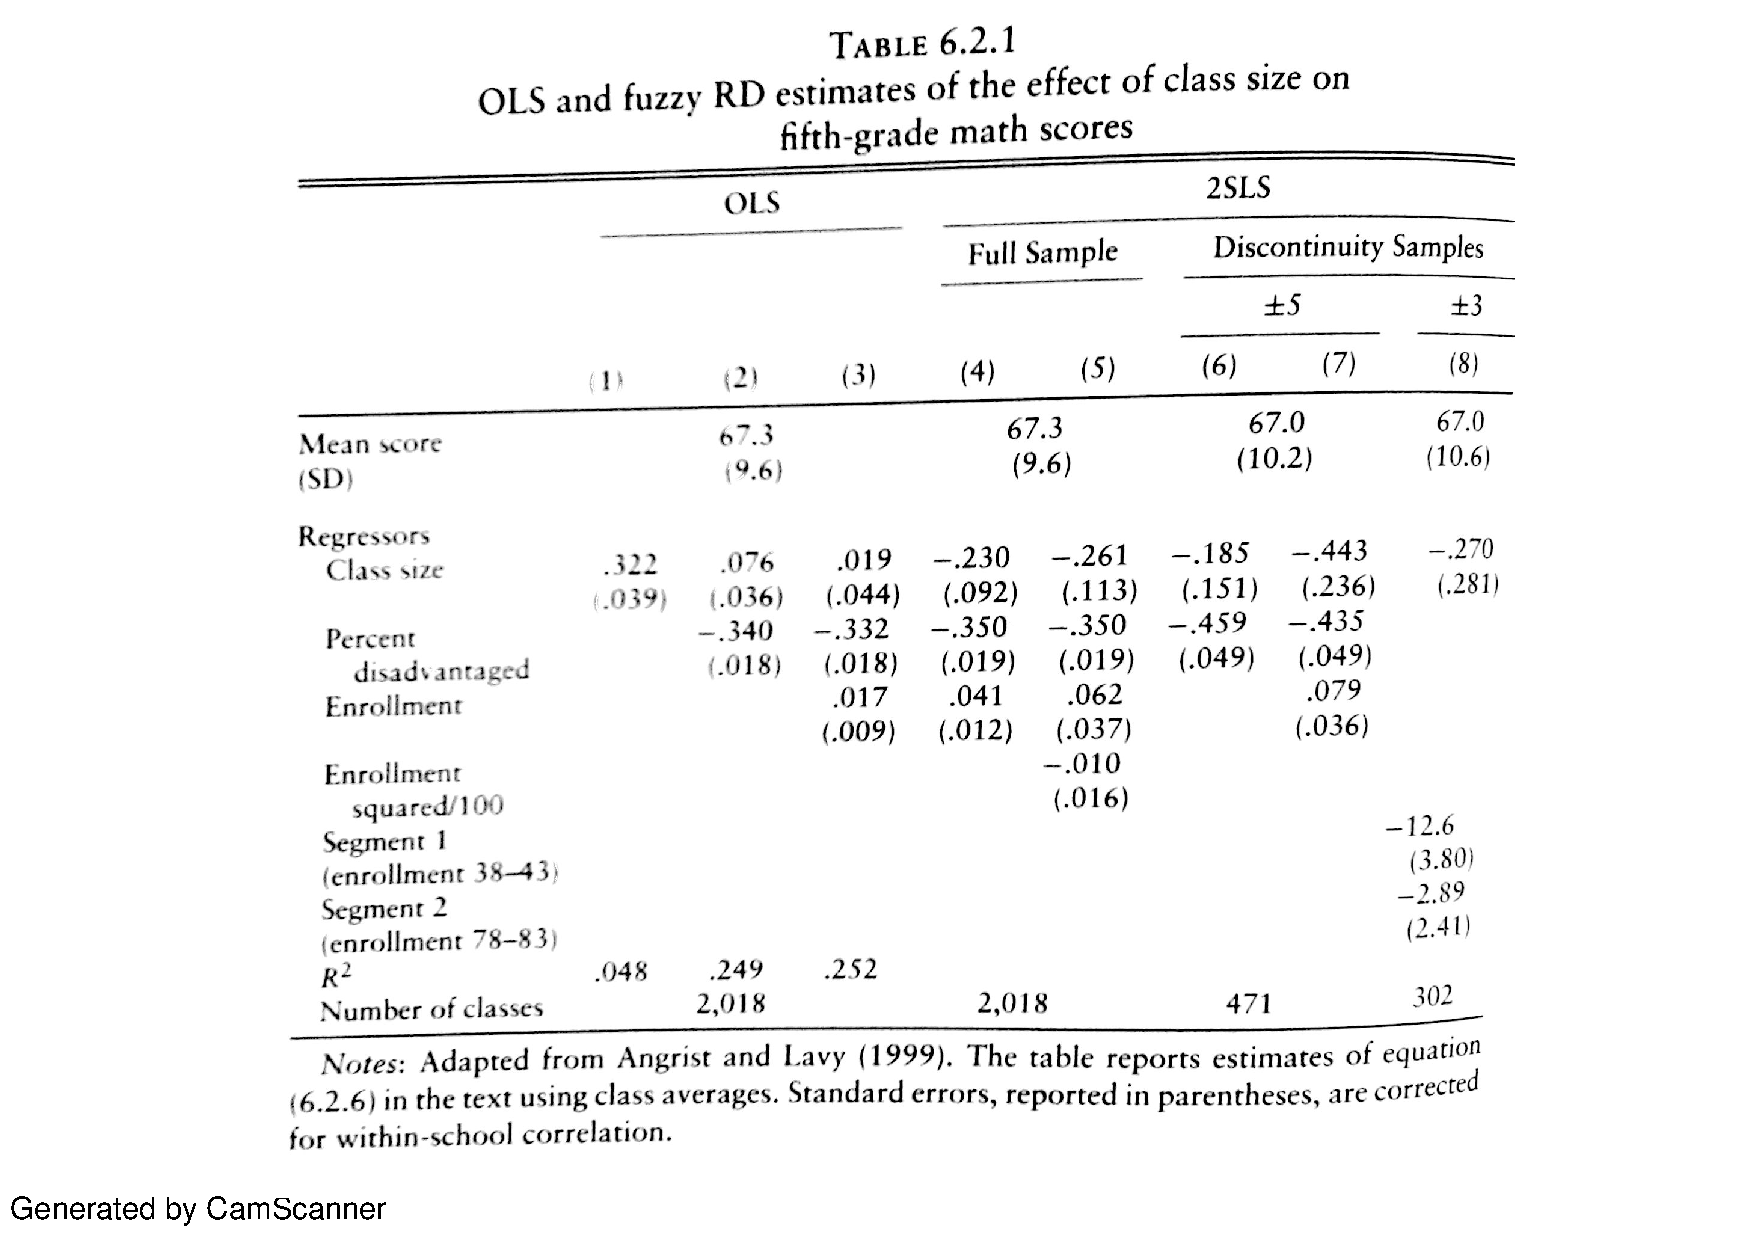
\includegraphics[width=\textwidth, trim=0.5in 0.3in 0.5in 0in, clip]{images/AngristPischkeTable621}
\end{figure}

\item Focusing on the math outcome (\textbf{avgmath}), estimate the OLS models (1,2,3) from Table 6.2.1. The relevant variables from the table are:
\begin{itemize}
\item \textbf{classize} : Class size
\item \textbf{tipuach} : Percent disadvantaged
\item \textbf{c\_size} : Enrollment (School cohort size)
\item \textbf{c\_size2} : $Enrollment^2/100$
\end{itemize}

Confirm that your coefficient estimates correspond with those reported in the table. Note: The SEs will differ from the published result, due to some procedures Angrist and Lavy used to address clustering of students within schools, which are unimportant for our purposes.

\item Conduct an additional test of conditional effects of class size given enrollment. By this, I mean that you should test whether the effect of class size is constant across different school enrollment cohort sizes (i.e., does class size have the same effect in schools less than 40 students as it does in schools with 40 to 80 students, etc.?).

To do this, create a new variable that takes a different value for each range of cohort sizes between the Maimonides discontinuities (i.e., your variable should be 1 if cohort size is between 0 and 40, 2 if cohort size is between 40 and 80, etc.). There are multiple ways to do this. Hint: look at the \texttt{cut()} function for the \texttt{egen} command. Use a scatterplot to confirm your new variable makes sense, and then estimate an OLS model of math scores on class size interacted with your new cohort variable. Does the marginal effect of class size vary across cohort sizes?

% egen cohortcut = cut(c_size), at(0, 40, 80, 120, 160, 200, 240)
% scatter cohortcut c_size
% reg avgmath c.classize##i.cohortcut
% margins, dydx(classize) over(cohortcut)


\item The instrument Angrist and Lavy use in this study is school enrollment, but as you've seen there are multiple discontinuities, so the endogenous variable (class size) is not a linear function of the instrument. You can (sort of) see this in a scatterplot (like Figure 6.2.1, panel A):\\
\texttt{twoway scatter classize c\_size}

\item This plot will probably be difficult to read. Consider the following code to see get a clearer picture. What does each step do?

\begin{verbatim}
snapshot save 1, label(``original'')
collapse (mean) classize, by(c_size)
scatter classize c_size
\end{verbatim}

You may also want to use the \texttt{lowess} command to draw a smoothed line through the scatterplot. This can be helpful for identifying potential discontinuities in a scatterplot. The command is used just like \texttt{scatter}. You may also want to use the \texttt{, bwidth()} option to adjust how the line is drawn. A small bandwidth value smooths over a narrower range of x-values (the default value is 1). Do you see the discontinuities? Restore the original data and try the same command on the original data.


\item To address the non-linear relationship between the instrument (enrollment) and class size, Angrist and Lavy calculate the class size expected by Maimonides' Rule as a function of school enrollment. This is stored as \textbf{func1}. Use a scatterplot to check for the linear of the relationship between this transformed version of the enrollment instrument and class size.

\item Using the \texttt{generate} command, transform \textbf{c\_size} into a new variable identical to \textbf{func1} that expresses Maimonides Rule.
% g func1= c_size/(int((c_size-1)/40)+1)

\item Use methods from earlier to assess instrument relevance.

\item Estimate the ``Full sample'' 2SLS models (4,5), instrumenting \texttt{classize} with \textbf{func1}.

\item Perform relevant postestimation commands.

\item One concern in a regression discontinuity approach is that the treatment (here class size) is only as if random right at the point of the discontinuity (or in this case, at the various discontinuities). In short, the previous results use the full sample data to estimate the effect of class size on test scores even though schools with, e.g., classes with 20 students or 105 students are not anywhere near the Maimonides' Rule thresholds (40, 80, 120, etc.). As a result, it is common in regression discontinuity designs to focus only on cases that are ``near'' the discontinuity threshold (i.e., within a particular bandwidth). The dataset contains a variable \textbf{disc} that is 1 if a student was in a school that had fell within 5 students of a threshold (e.g., between 36 and 45). To get a sense of this subsample indicator variable, use \texttt{tab} and \texttt{twoway scatter disc c\_size} to see which students are included in this causally more credible subsample.

\item Using the \texttt{if} statement to subset the data during estimation, estimate the ``discontinuity sample'' models (6,7).

\item The last column of Table 6.2.1 uses an even narrower subset of students (those within 3 students of discontinuity threshold). Generate a new variable \textbf{disc3} that serves as an indicator for these students. Additionally, you need to create indicators for which group the student is in. With those three variables, run the 2SLS estimate shown in the last column. Don't worry if your results don't match exactly but you should be able to match them to within about 0.1.

\item Repeat the previous exercise with other bandwidths (of your choice) around the discontinuities.

\item You can repeat the above analyses using \textbf{avgverb} as the outcome.

\end{enumerate}


\end{document}